\documentclass[11pt]{article}
\usepackage[a4paper,margin=2.2cm]{geometry}
\usepackage{amsmath,amssymb,booktabs,graphicx,xcolor,array,enumitem}
\usepackage[hidelinks]{hyperref}
\usepackage[section]{placeins}
\graphicspath{{../figures/8/}{../figures/}}
% generated by 11_paper.py; do not edit
\newcommand{\nGapFrac}{16.5}
\newcommand{\nGapFracUnc}{2.5}
\newcommand{\nGapFracDec}{0.165}
\newcommand{\nCTrue}{6.07}
\newcommand{\nNToys}{2000}
\newcommand{\nNHqeToys}{12000}
\newcommand{\nInclMeanMx}{4.568}
\newcommand{\nInclVarMx}{1.62}
\newcommand{\nInclVarMxUnc}{0.08}
\newcommand{\nInclMeanEl}{1.390}
\newcommand{\nInclVarEl}{0.185}
\newcommand{\nInclMeanQ}{4.399}
\newcommand{\nInclVarQ}{7.93}
\newcommand{\nSemMeanMx}{4.32}
\newcommand{\nSemVarMx}{1.22}
\newcommand{\nSemMeanEl}{1.41}
\newcommand{\nSemMeanQ}{4.42}
\newcommand{\nGapMeanMx}{5.83}
\newcommand{\nGapMeanMxLo}{5.35}
\newcommand{\nGapMeanMxHi}{6.30}
\newcommand{\nGapMeanEl}{1.30}
\newcommand{\nGapMeanQ}{4.27}
\newcommand{\nDMeanMx}{0.25}
\newcommand{\nFMinTwoMoment}{0.11}
\newcommand{\nShareD}{24.6}
\newcommand{\nShareDst}{57.2}
\newcommand{\nShareDss}{14.8}
\newcommand{\nShareDpipi}{3.1}
\newcommand{\nShareDsK}{0.3}
\newcommand{\nClosureLOneLo}{0.02}
\newcommand{\nClosureLOneHi}{0.08}
\newcommand{\nClosureOutMxLo}{21}
\newcommand{\nClosureOutMxHi}{66}
\newcommand{\nClosureOutQDstEta}{37}
\newcommand{\nClosureBfGapMxLo}{7}
\newcommand{\nClosureBfGapMxHi}{8}
\newcommand{\nClosureBfGapQLo}{15}
\newcommand{\nClosureBfGapQHi}{21}
\newcommand{\nGapAllowedMx}{74}
\newcommand{\nInclAllowed}{100}
\newcommand{\nCdfMxEightLo}{0.74}
\newcommand{\nCdfMxTenLo}{0.93}
\newcommand{\nCdfMxTenLoToys}{0.88}
\newcommand{\nCdfMxTenLoPct}{93}
\newcommand{\nCdfElHalfHi}{0.16}
\newcommand{\nCdfElHalfHiToys}{0.17}
\newcommand{\nAboveElEight}{60}
\newcommand{\nCdfQFourLo}{0.19}
\newcommand{\nCdfQFourHi}{0.79}
\newcommand{\nCdfQSixLo}{0.40}
\newcommand{\nCdfQSixLoToys}{0.36}
\newcommand{\nLcpOutMx}{95}
\newcommand{\nLcpOutQ}{17}
\newcommand{\nLcpEdgeMx}{10.4}
\newcommand{\nLcpEdgeQ}{4.2}
\newcommand{\nLcpAllowedMx}{0}
\newcommand{\nDskAllowedMx}{8}
\newcommand{\nGapLimitMx}{0.065}
\newcommand{\nGapLimitMxPct}{6.5}
\newcommand{\nGapLimitEl}{0.035}
\newcommand{\nToyFracNominal}{79}
\newcommand{\nToyFracHalfAt}{0.13}
\newcommand{\nToyFracAtSeven}{0.5}
\newcommand{\nShapeSemMx}{41.9}
\newcommand{\nShapeDMx}{93.6}
\newcommand{\nShapeDstMx}{70.1}
\newcommand{\nShapeDssMx}{2.2}
\newcommand{\nShapeDpipiMx}{24.7}
\newcommand{\nShapeDsKMx}{92.1}
\newcommand{\nShapeSemEl}{13.9}
\newcommand{\nShapeDEl}{9.7}
\newcommand{\nShapeDstEl}{40.3}
\newcommand{\nShapeDssEl}{5.9}
\newcommand{\nShapeDpipiEl}{37.5}
\newcommand{\nShapeDsKEl}{53.2}
\newcommand{\nShapeSemQ}{5.7}
\newcommand{\nShapeDQ}{11.2}
\newcommand{\nShapeDstQ}{19.1}
\newcommand{\nShapeDssQ}{32.5}
\newcommand{\nShapeDpipiQ}{36.1}
\newcommand{\nShapeDsKQ}{34.6}
\newcommand{\nShapeSemAll}{168}
\newcommand{\nShapeDAll}{242}
\newcommand{\nShapeDstAll}{194}
\newcommand{\nShapeDssAll}{229}
\newcommand{\nShapeDpipiAll}{207}
\newcommand{\nShapeDsKAll}{250}
\newcommand{\nShapeSemP}{<0.001}
\newcommand{\nShapeDP}{<0.001}
\newcommand{\nShapeDstP}{<0.001}
\newcommand{\nShapeDssP}{<0.001}
\newcommand{\nShapeDpipiP}{<0.001}
\newcommand{\nShapeDsKP}{<0.001}
\newcommand{\nShapeFreeLo}{150}
\newcommand{\nShapeFreeHi}{168}
\newcommand{\nPhspDsq}{20.4}
\newcommand{\nPhspP}{0.003}
\newcommand{\nPhspRejFrac}{100}
\newcommand{\nBareDsq}{10.1}
\newcommand{\nBareP}{0.013}
\newcommand{\nPhspInclP}{0.020}
\newcommand{\nBareInclP}{0.038}
\newcommand{\nGInclUnc}{1.41}
\newcommand{\nLineshapeAllowed}{allowed}
\newcommand{\nWrongSupportDsq}{28.7}

\newcommand{\GeV}{\,\mathrm{GeV}}
\newcommand{\Mx}{M_X^2}
\newcommand{\El}{E_\ell}
\newcommand{\Lcp}{\Lambda_c\bar p}
\newcommand{\BR}{\mathcal{B}}
\setlist{itemsep=1pt,topsep=3pt}
\title{Narrative}
\author{}
\date{15 October 2026}
\begin{document}
\maketitle
\vspace{-1.5em}

\section*{Summary}
The known exclusive modes (SEM) add up to $\nGapFrac\%$ less than the inclusive $B\to X_c\ell\nu$ rate. We call the
missing part the gap. We assume only that the gap has a positive spectrum and combine this with the zero-threshold
moments of $\Mx$, $\El$ and $q^2$ from the HQE fit. Three results follow.
\begin{enumerate}
\item \textbf{The gap is not more of the known modes.} The inclusive moments cannot be described by the SEM with its
  branching fractions scaled up, neither by one common factor nor by any single mode. The gap is heavier in $\Mx$ (mean
  $\nGapMeanMx$ vs $\nSemMeanMx\GeV^2$) and softer in $\El$ ($\nGapMeanEl$ vs $\nSemMeanEl\GeV$) than the SEM, but
  SEM-like in $q^2$.
\item \textbf{Positivity limits where the gap can be and how big it is.} At least $\nCdfMxTenLoPct\%$ of the gap lies
  below $\Mx = 10\GeV^2$, so $\Lcp\ell\nu$ cannot be the whole gap. The gap must be at least $\nGapLimitMxPct\%$ of the
  inclusive rate ($95\%$ CL).
\item \textbf{The $\Mx$ moments check MC lineshapes.} $D^{(*)}\pi\pi\ell\nu$ with a phase-space lineshape is rejected
  ($p = \nPhspP$), and so are EvtGen broad $D^{**}$ lineshapes without the MCAmbulance correction ($p = \nBareP$). The
  Belle~II cocktail passes.
\end{enumerate}
All statements assume the HFLAV branching fractions of the SEM.

\section{Method}

\FloatBarrier
\subsection{Inclusive input}
The inclusive input is the HQE fit to the measured moments (arXiv:2609.28752). The fit describes the moments measured
above a threshold on $\El$ or $q^2$ and extrapolates them to the full phase space (zero threshold, Fig.~\ref{fig:hqe}).
This gives the first three moments of $\Mx$, of the lepton energy $\El$ in the $B$ rest frame, and of $q^2$, with
$\nNHqeToys$ likelihood toys that carry all experimental and theory uncertainties and correlations. The means and
variances are $\langle\Mx\rangle = \nInclMeanMx\GeV^2$, $\mathrm{Var}(\Mx) = \nInclVarMx\pm\nInclVarMxUnc\GeV^4$;
$\langle\El\rangle = \nInclMeanEl\GeV$, $\mathrm{Var}(\El) = \nInclVarEl\GeV^2$; $\langle q^2\rangle = \nInclMeanQ\GeV^2$,
$\mathrm{Var}(q^2) = \nInclVarQ\GeV^4$.
\begin{figure}[htbp]\centering
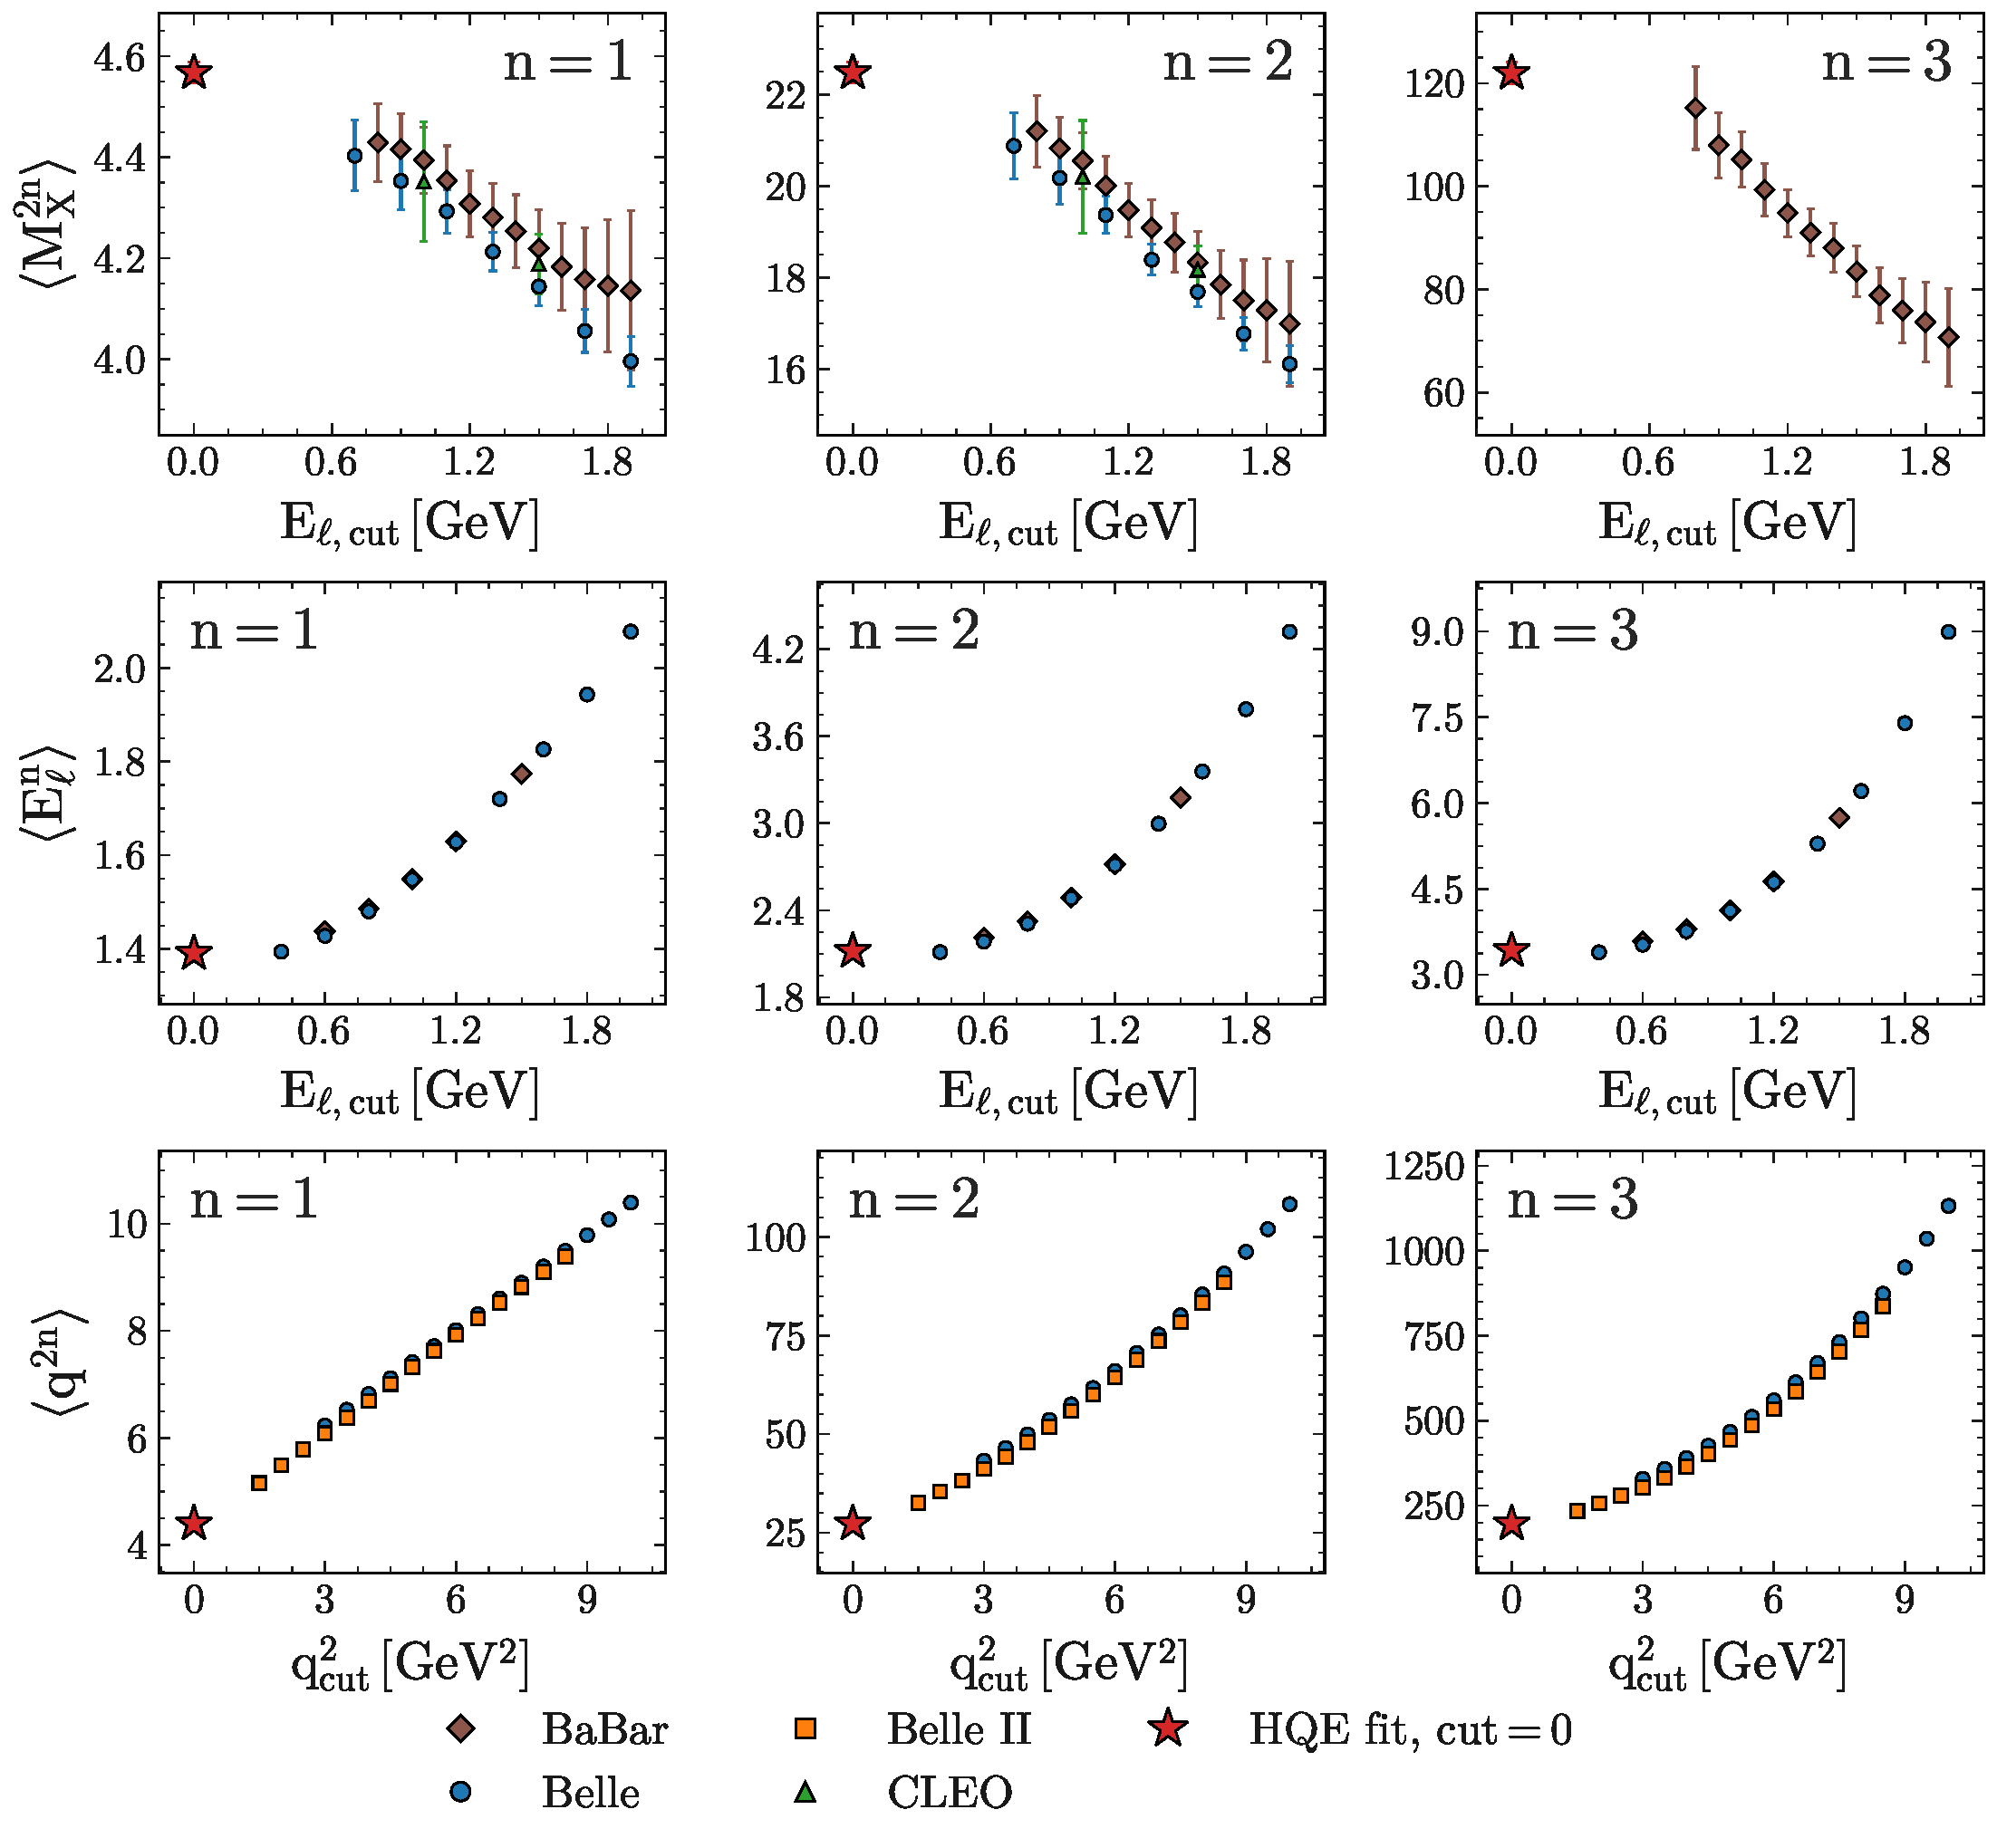
\includegraphics[width=0.75\linewidth]{hqe_moments.pdf}
\caption{Measured raw moments $\langle x^n\rangle$ as a function of the threshold, and the HQE fit extrapolated to zero
threshold (star), which is the inclusive input.}\label{fig:hqe}
\end{figure}

\FloatBarrier
\subsection{Sum of exclusives}
The SEM is the Belle~II analysis cocktail, generated with EvtGen (basf2 \texttt{release-09-00-11}) for $B^+$ and $B^0$,
electrons and muons, and reweighted with Hammer:
\begin{itemize}
\item $B\to D\ell\nu$ and $D^*\ell\nu$: BLPRXP form factors (one fit for both, shared eigenvariations).
\item $B\to D^{**}\ell\nu$ ($D_0^*$, $D_1'$, $D_1$, $D_2^*$): BLR form factors. The broad $D_0^*$ and $D_1'$ get the
  MCAmbulance correction of their lineshape, which removes unphysical high-mass tails.
\item $B\to D^{(*)}\pi\pi\ell\nu$: generated through the broad $D_1'$ and $D_0^*$ (50:50) decaying to
  $D^{(*)}\pi\pi$, with the same corrections.
\item $B\to D_s^{(*)}K\ell\nu$: phase space, reweighted to the measured spectrum.
\end{itemize}
Branching fractions are from HFLAV. The SEM adds up to $\BR = 9.26\%$ ($B^+$) and $8.55\%$ ($B^0$), shared as $D$
$\nShareD\%$, $D^*$ $\nShareDst\%$, $D^{**}$ $\nShareDss\%$, $D^{(*)}\pi\pi$ $\nShareDpipi\%$ and $D_s^{(*)}K$
$\nShareDsK\%$. With the HFLAV inclusive rate the gap is $1.79\%$ ($B^+$) and $1.72\%$ ($B^0$), i.e.\
$\BR_\text{gap}/\BR_\text{incl} = (\nGapFrac\pm\nGapFracUnc)\%$.

\FloatBarrier
\subsection{Gap moments}
For each observable the raw gap moments follow from the inclusive and SEM moments,
\begin{equation*}
m_k^\text{gap} = c\, m_k^\text{incl} - (c-1)\, m_k^\text{SEM}, \qquad c = \BR_\text{incl}/\BR_\text{gap} = \nCTrue .
\end{equation*}
The factor $c$ amplifies any difference between the inclusive and SEM spectra six-fold, which is why the gap moments are
sensitive to small details of the SEM.

\FloatBarrier
\subsection{Uncertainties}
We use $\nNToys$ toys. Each toy varies the SEM (MC statistics, form-factor eigenvariations, branching fraction of each
mode), the gap normalisation $\BR_\text{gap}$ (fully correlated across $B^+$, $B^0$ and lepton flavours), and draws one
HQE likelihood toy. Table~\ref{tab:budget} gives the resulting relative uncertainties of the gap moments. The form
factors dominate $\Mx$; the branching fractions per mode dominate $q^2$.
\begin{table}[htbp]\centering\small
\input{../output/6/moment_budget_data_thr0.tex}
\caption{Relative uncertainty of the gap moments $m_{1..3}$ by source, in percent.}\label{tab:budget}
\end{table}

\FloatBarrier
\subsection{Positivity test}
The moments of a positive spectrum on a finite range must satisfy a set of inequalities (the Hausdorff moment problem).
We use $\Mx\in[3.2, 16]\GeV^2$, $\El\in[0, 2.3]\GeV$ and $q^2\in[0, 11.7]\GeV^2$. The test statistic is the $\chi^2$
distance $d^2 = \Delta^T V^{-1}\Delta$ from the gap moments to the nearest moments a positive spectrum can have, with
$V$ the toy covariance; $d^2 = 0$ if the moments are allowed. The $p$-value is the fraction of toys, centred on that
nearest point, that reach a larger $d^2$ (the toys are not Gaussian, so we do not use the $\chi^2$ formula). The same
$d^2$ also compares two sets of moments directly; if they agree it is about the number of moments compared, 3 per
observable and 9 for all three.

To display a spectrum with given moments we use the maximum-entropy (MaxEnt) density, the smoothest positive density
with those moments, optionally with the known behaviour at the kinematic endpoints of $\El$ and $q^2$. It is an
illustration; no quantitative result uses it.

\FloatBarrier
\subsection{Validation}
We inject two known gaps into the SEM, build the gap moments as above, and reconstruct the gap spectrum
(Fig.~\ref{fig:closure}). For $D_1'\to D^*\eta$ and for $50\%\,D\ell\nu + 50\%\,\Lcp\ell\nu$, the reconstructions follow
the true spectra in $\El$ and $q^2$ ($L_1$ distance $\nClosureLOneLo$--$\nClosureLOneHi$). $\Mx$ is the weakest
observable: three moments cannot describe a narrow peak next to a broad continuum, and fluctuations push the moments
outside the allowed region in $\nClosureOutMxLo$--$\nClosureOutMxHi\%$ of the toys even though the true gap is positive.
The same happens in $q^2$ for the narrow $D^*\eta$ gap ($\nClosureOutQDstEta\%$ of the toys). The leading uncertainty is
the gap normalisation $\BR_\text{gap}$ ($\nClosureBfGapMxLo$--$\nClosureBfGapMxHi\%$ on $m_1$ of $\Mx$,
$\nClosureBfGapQLo$--$\nClosureBfGapQHi\%$ on $m_1$ of $q^2$), followed by the branching fractions per mode and the form
factors; the HQE moments and the MC statistics are small.
\begin{figure}[htbp]\centering
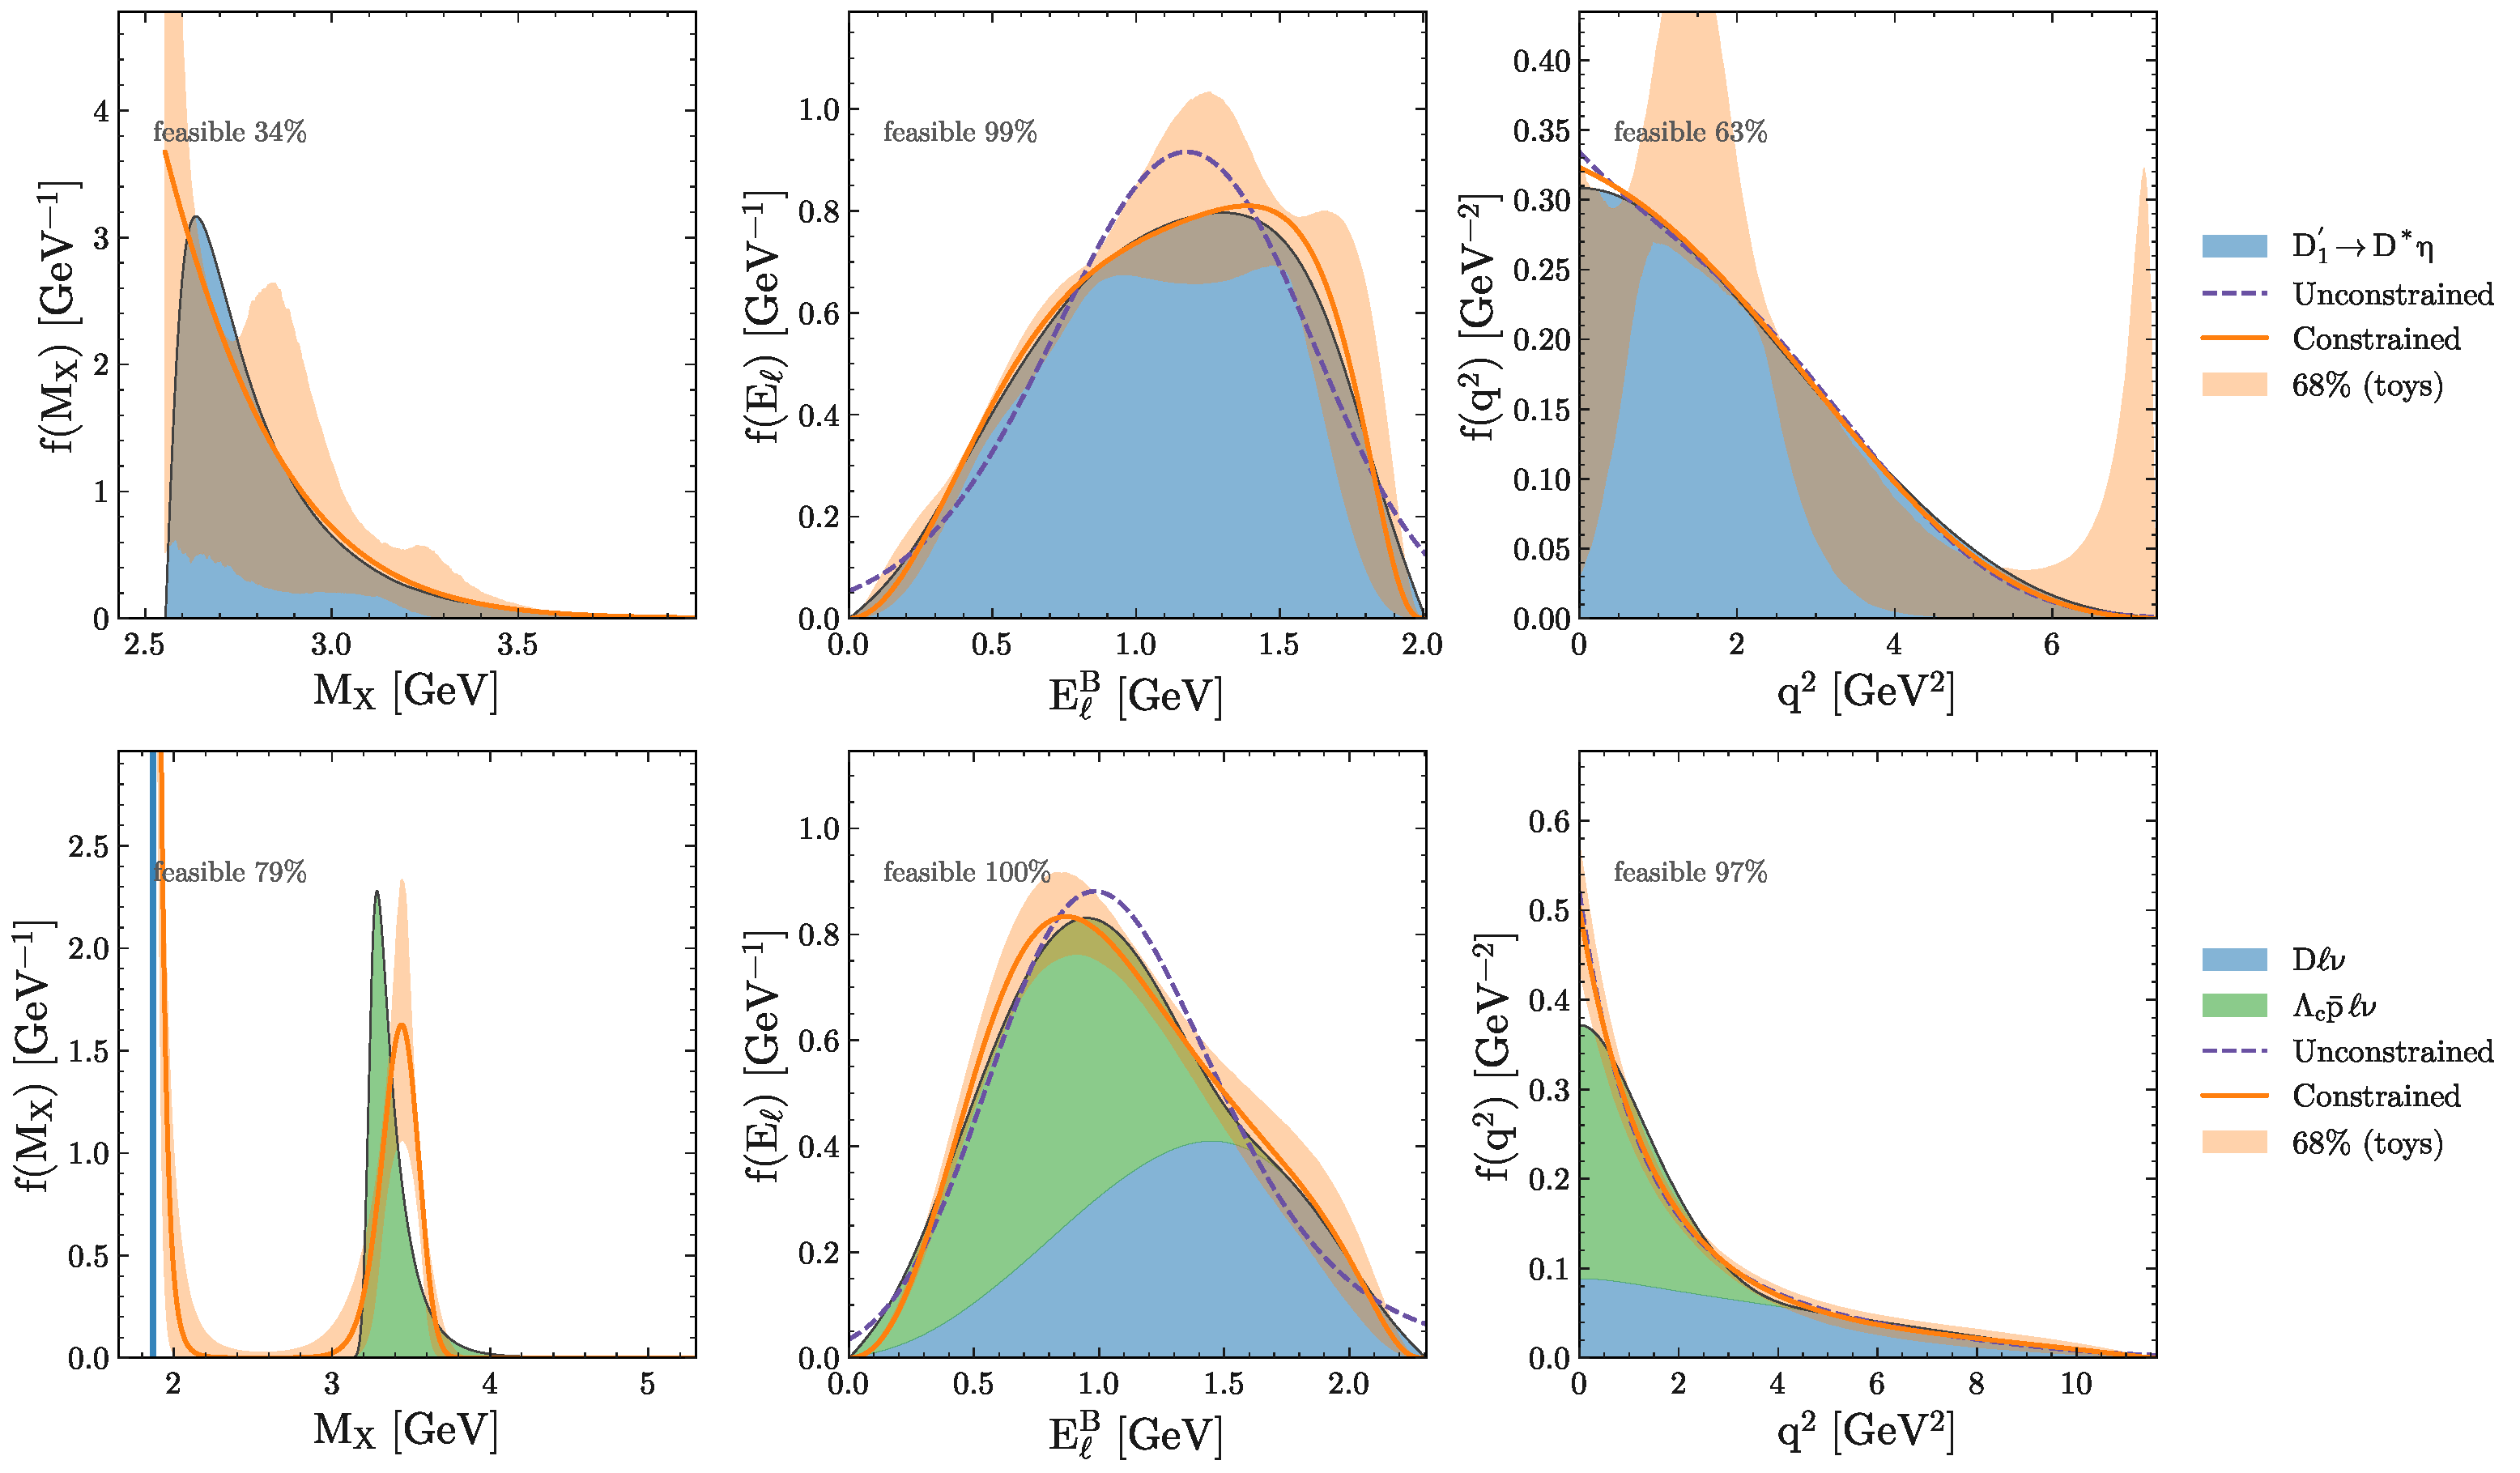
\includegraphics[width=\linewidth]{closure_n3.pdf}
\caption{Closure test with three moments. Top: injected gap $D_1'\to D^*\eta$; bottom: $50\%\,D\ell\nu +
50\%\,\Lcp\ell\nu$. Filled: true gap. Lines: MaxEnt reconstruction without (dashed) and with (solid) endpoint
behaviour; band: $68\%$ of the toys. ``Feasible'': fraction of toys whose gap moments a positive spectrum can have.}
\label{fig:closure}
\end{figure}

\section{Results}

\FloatBarrier
\subsection{Inclusive spectrum vs the SEM}
Before subtracting anything, we invert the inclusive moments alone and compare the result with the SEM, both normalised
to unit area (Fig.~\ref{fig:incl}). This needs neither $c$ nor the gap normalisation. The inclusive moments are allowed
in $\nInclAllowed\%$ of the toys for all three observables. In $\El$ the inclusive spectrum is slightly softer than the
SEM: it lies above the SEM below about $1.4\GeV$. In $q^2$ the two agree to within a few percent. In $\Mx$ three moments
cannot resolve the $D$ and $D^*$ lines, so the inversion is only a smooth curve; there the comparison is made on the
moments. The differences are small by eye; the factor $c\approx6$ turns them into the gap.
\begin{figure}[htbp]\centering
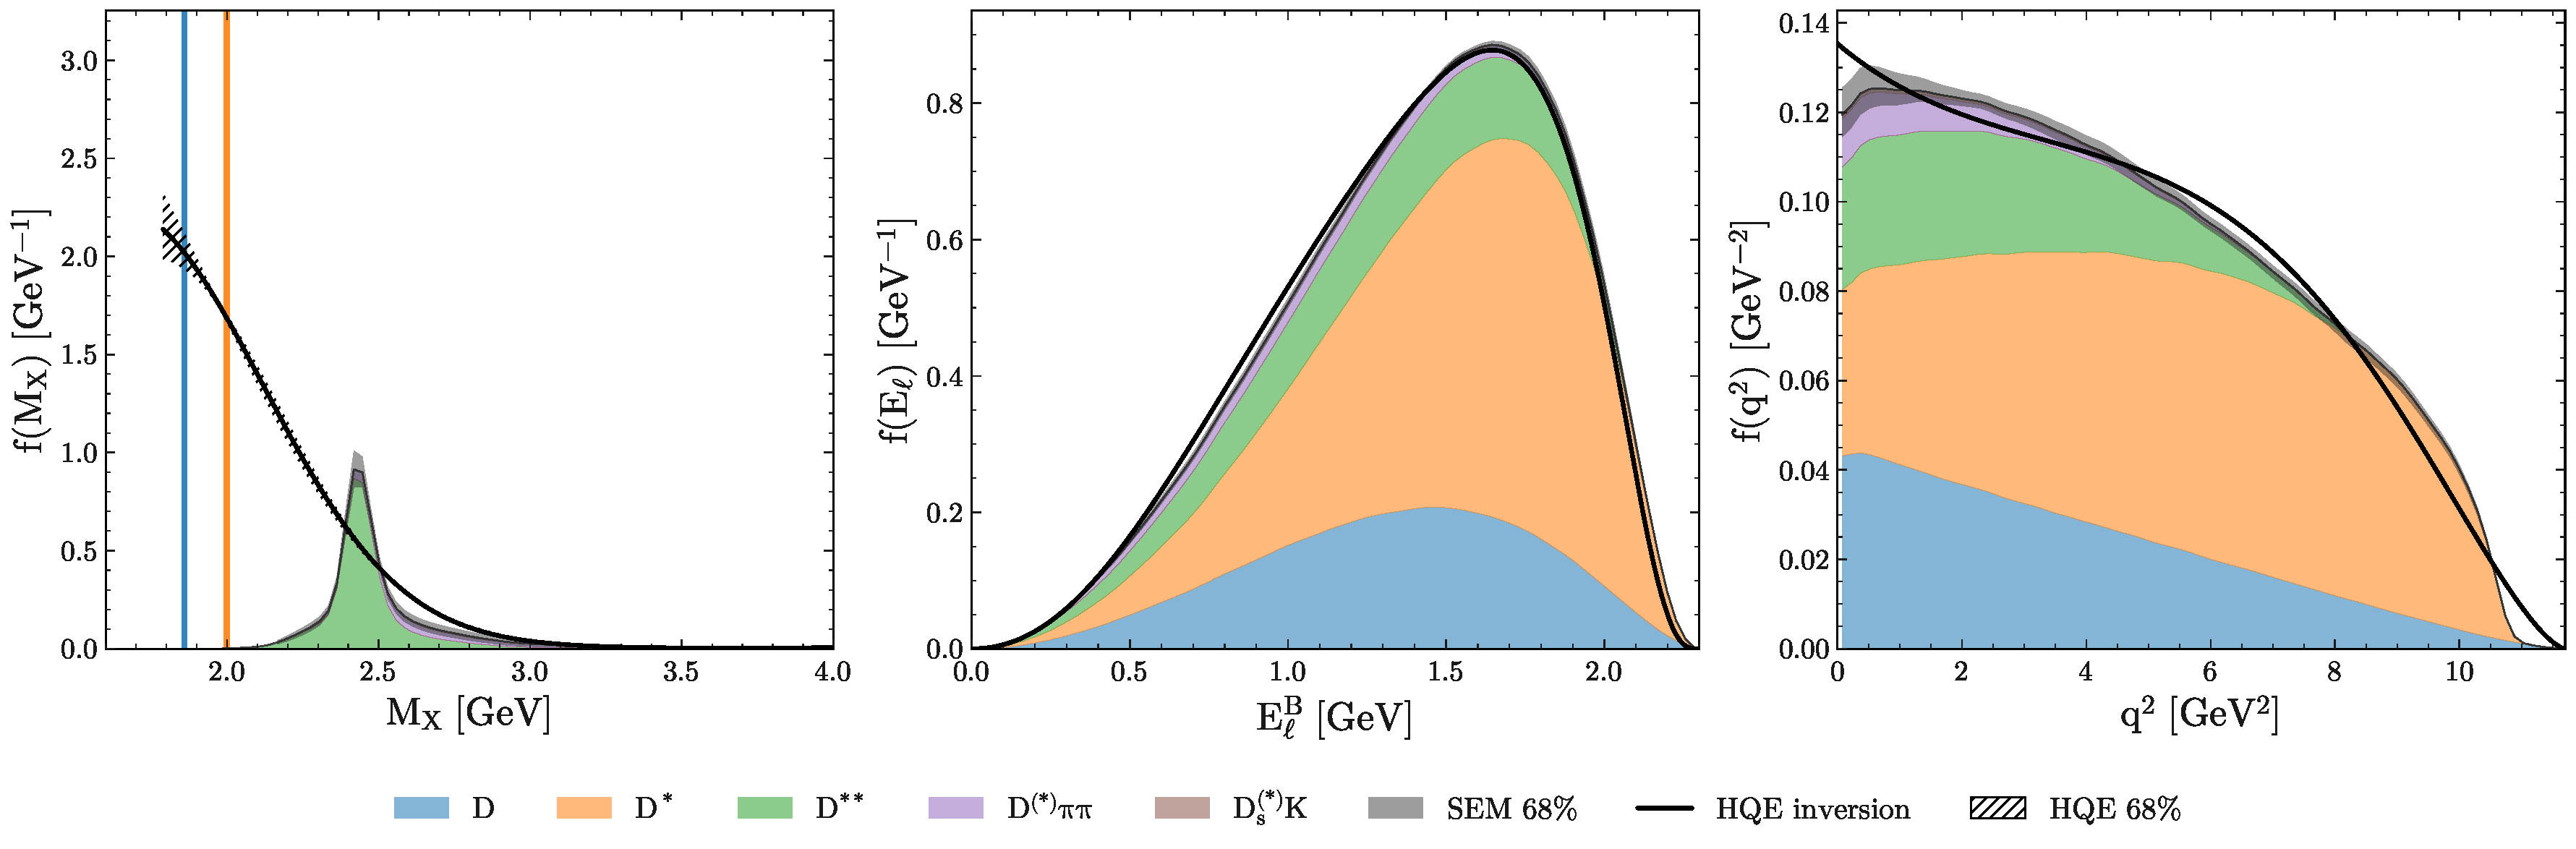
\includegraphics[width=\linewidth]{6/hqe_vs_sem_stack.pdf}
\caption{MaxEnt inversion of the inclusive HQE moments without SEM subtraction (black, hatched: $68\%$ of the HQE
toys), against the SEM stacked by mode (grey band: $68\%$ of the SEM toys). Both are normalised to unit area. Vertical
lines in $M_X$: the $D$ and $D^*$ masses.}\label{fig:incl}
\end{figure}

\FloatBarrier
\subsection{The gap spectrum}
Figure~\ref{fig:gap} shows the MaxEnt reconstruction of the gap from the measured moments. In $\Mx$ the gap is a broad
bump at $M_X\approx2.4\GeV$, above the $D$ and $D^*$ masses and around the $D^{**}$ states. In $\El$ it peaks near
$1.45\GeV$ and extends down to about $0.3\GeV$. In $q^2$ it falls slowly over the full range. The gap moments are
allowed for all three observables: in $\nGapAllowedMx\%$ of the toys for $\Mx$ and in all toys for $\El$ and $q^2$.
\begin{figure}[htbp]\centering
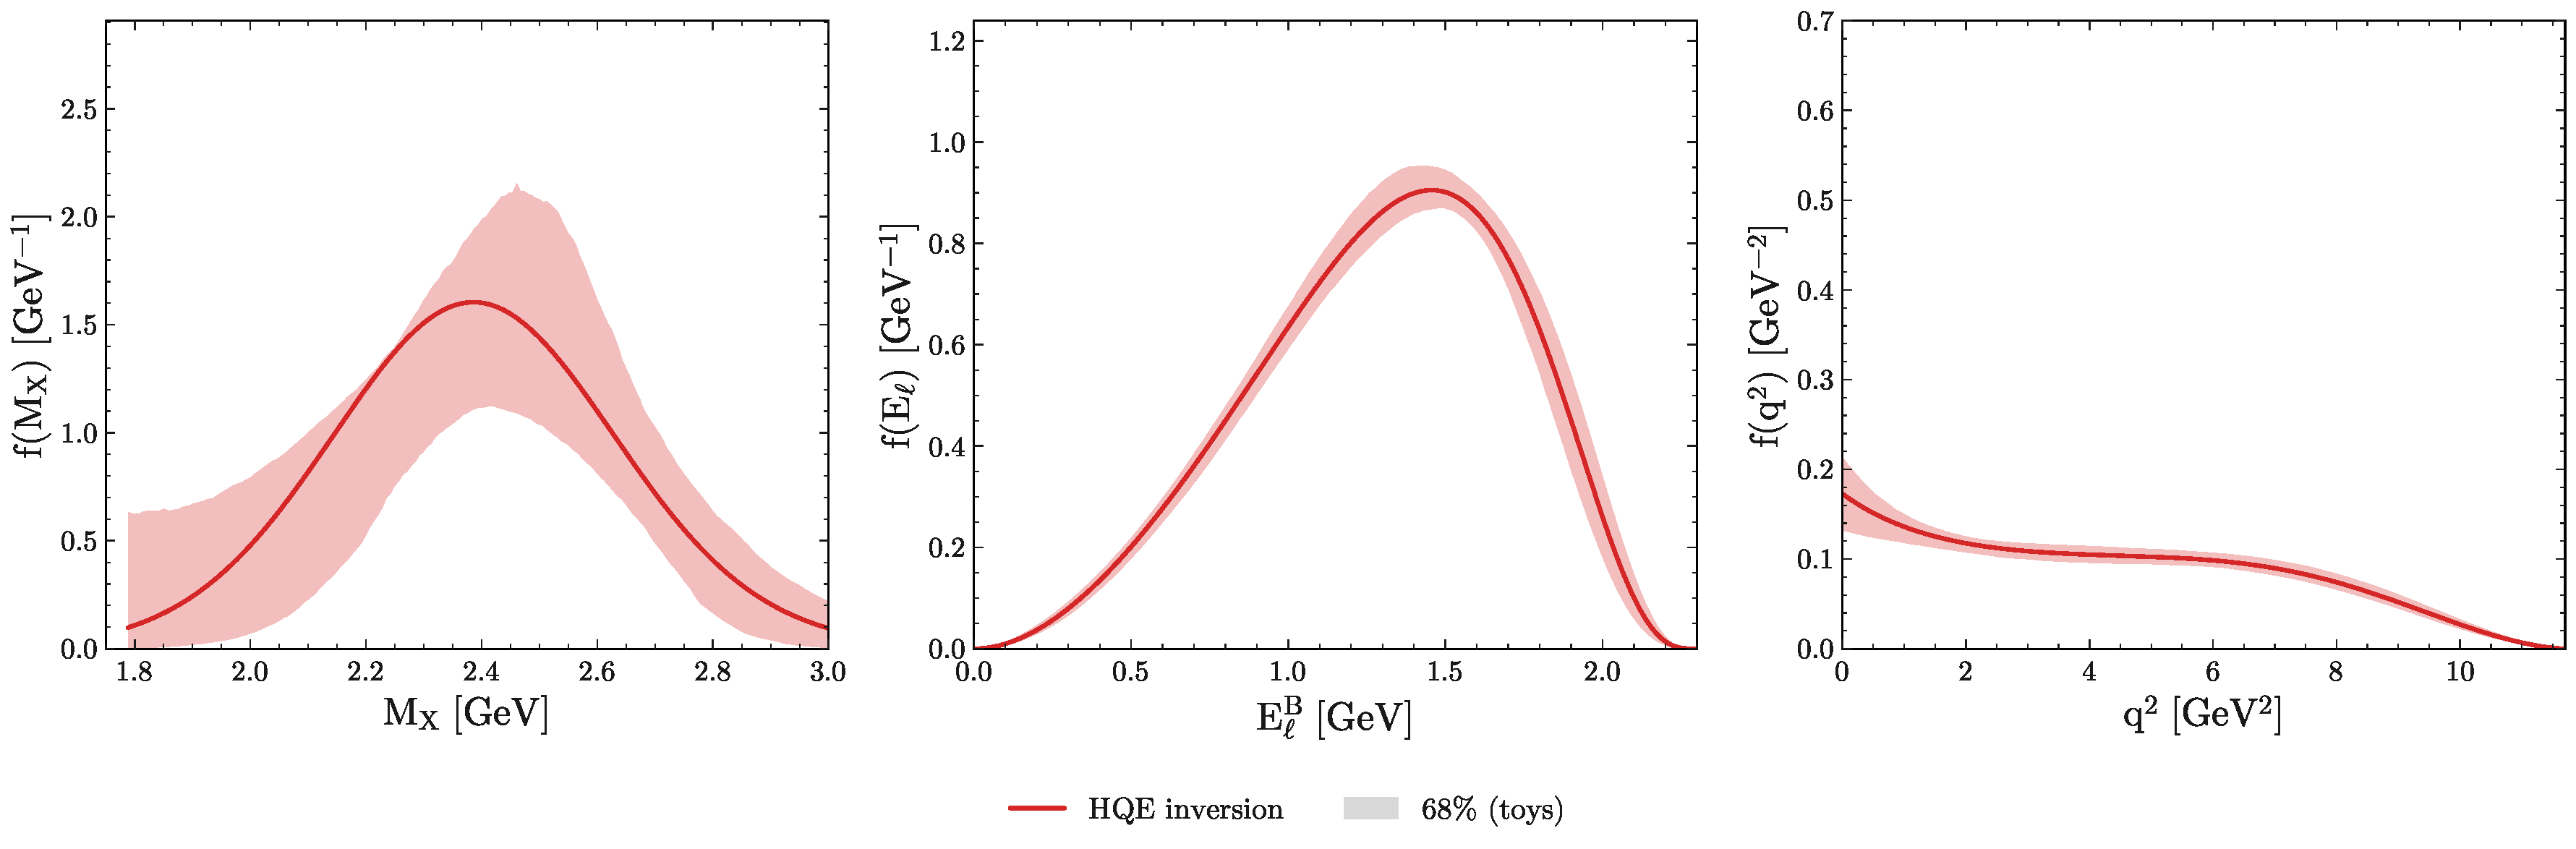
\includegraphics[width=\linewidth]{6/gap_density.pdf}
\caption{MaxEnt reconstruction of the gap from three moments per observable, with endpoint behaviour for $\El$ and
$q^2$; band: $68\%$ of the toys. Illustration only.}\label{fig:gap}
\end{figure}

\FloatBarrier
\subsection{The gap is not more of the known modes}
Could the gap simply be the known modes with larger branching fractions? Then the inclusive spectrum would be the SEM
plus extra rate with the shape of one SEM mode. We compare the inclusive moments with such models directly,
using $d^2$ (Table~\ref{tab:shape}); $d^2\approx3$ per observable and $\approx9$ for all three if a model fits. Unlike
the gap moments, this comparison is not multiplied by $c$: the inclusive moments are compared as measured. The gap size
enters only as the amount of extra rate, at its nominal value $\BR_\text{gap}/\BR_\text{incl} = \nGapFracDec$, or left
free.
\begin{table}[htbp]\centering\small
\begin{tabular}{lccccc}
\toprule
Gap shaped like \ldots & $\Mx$ & $\El$ & $q^2$ & all three & $p$ (all three) \\
\midrule
the whole SEM (common factor, any size) & \nShapeSemMx & \nShapeSemEl & \nShapeSemQ & \nShapeSemAll & $\nShapeSemP$ \\
$D\ell\nu$ & \nShapeDMx & \nShapeDEl & \nShapeDQ & \nShapeDAll & $\nShapeDP$ \\
$D^*\ell\nu$ & \nShapeDstMx & \nShapeDstEl & \nShapeDstQ & \nShapeDstAll & $\nShapeDstP$ \\
$D^{**}\ell\nu$ & \nShapeDssMx & \nShapeDssEl & \nShapeDssQ & \nShapeDssAll & $\nShapeDssP$ \\
$D^{(*)}\pi\pi\ell\nu$ & \nShapeDpipiMx & \nShapeDpipiEl & \nShapeDpipiQ & \nShapeDpipiAll & $\nShapeDpipiP$ \\
$D_s^{(*)}K\ell\nu$ & \nShapeDsKMx & \nShapeDsKEl & \nShapeDsKQ & \nShapeDsKAll & $\nShapeDsKP$ \\
\bottomrule
\end{tabular}
\caption{$d^2$ between the inclusive moments and the SEM plus a gap with the shape of one SEM mode, at the nominal gap
size. $p$ from toys; $<0.001$ means no toy reached the observed $d^2$. The joint $d^2$ exceeds the sum of the three
because the observables are correlated.}\label{tab:shape}
\end{table}

No single mode works. Leaving the gap size free does not rescue any of them: the best fits shrink the extra rate
towards zero and end at joint $d^2 = \nShapeFreeLo$--$\nShapeFreeHi$. Figure~\ref{fig:plane} shows why. In $\Mx$ and
$\El$ the gap sits near the $D^{**}$, but in $q^2$ every heavy mode lies far below the gap, which sits on top of the
SEM. The nearest single mode, $D^{**}$, fits $\Mx$ and $\El$ but fails in $q^2$ ($d^2 = \nShapeDssQ$). For reference,
Fig.~\ref{fig:plane_cand} shows the same plane with candidate gap modes outside the SEM.
\begin{figure}[htbp]\centering
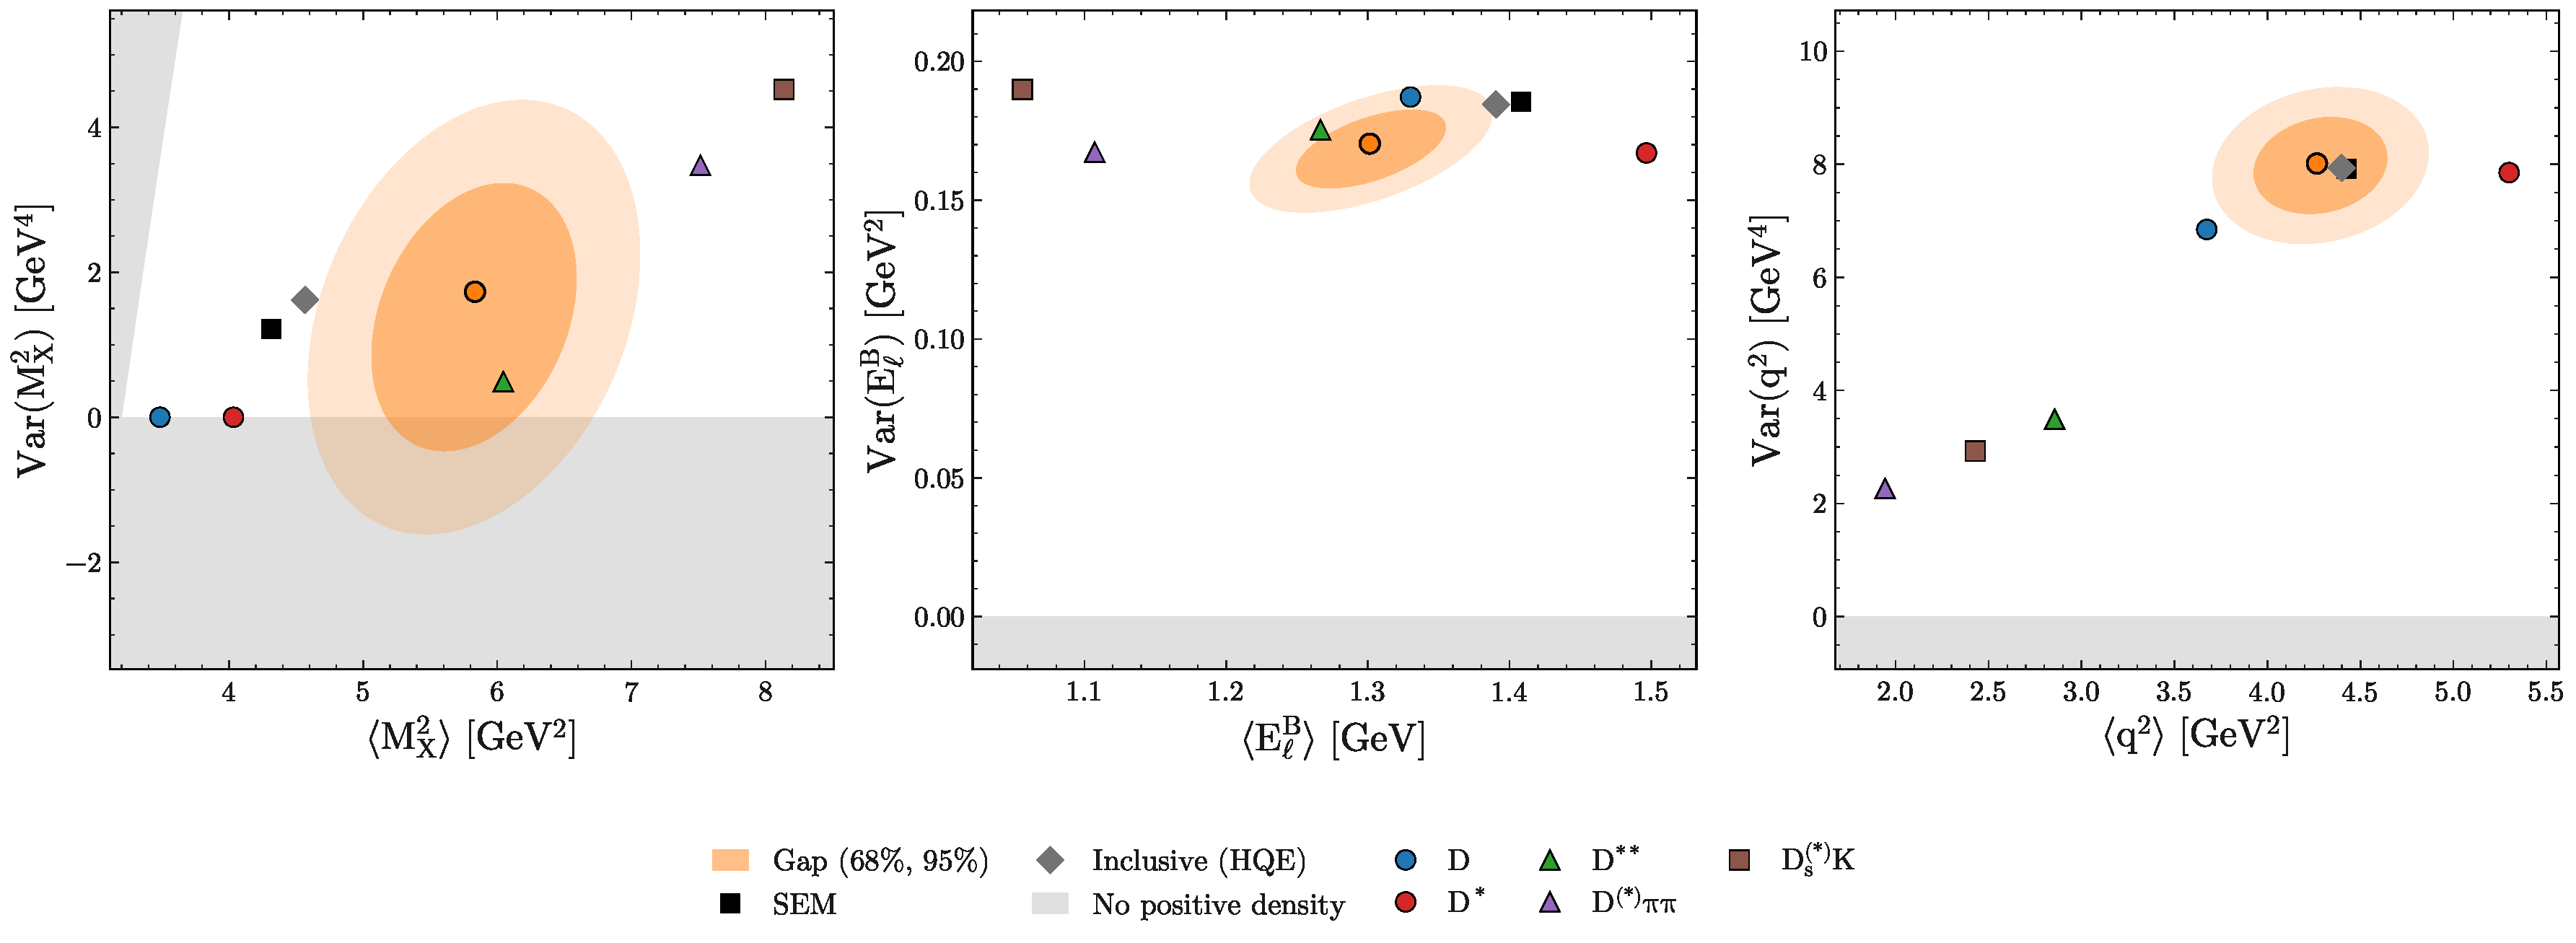
\includegraphics[width=\linewidth]{moment_plane_sem.pdf}
\caption{Mean vs variance of the gap ($68\%$, $95\%$ of the toys), of the SEM, of the inclusive moments and of each SEM
mode. Grey: no positive spectrum possible.}\label{fig:plane}
\end{figure}
\begin{figure}[htbp]\centering
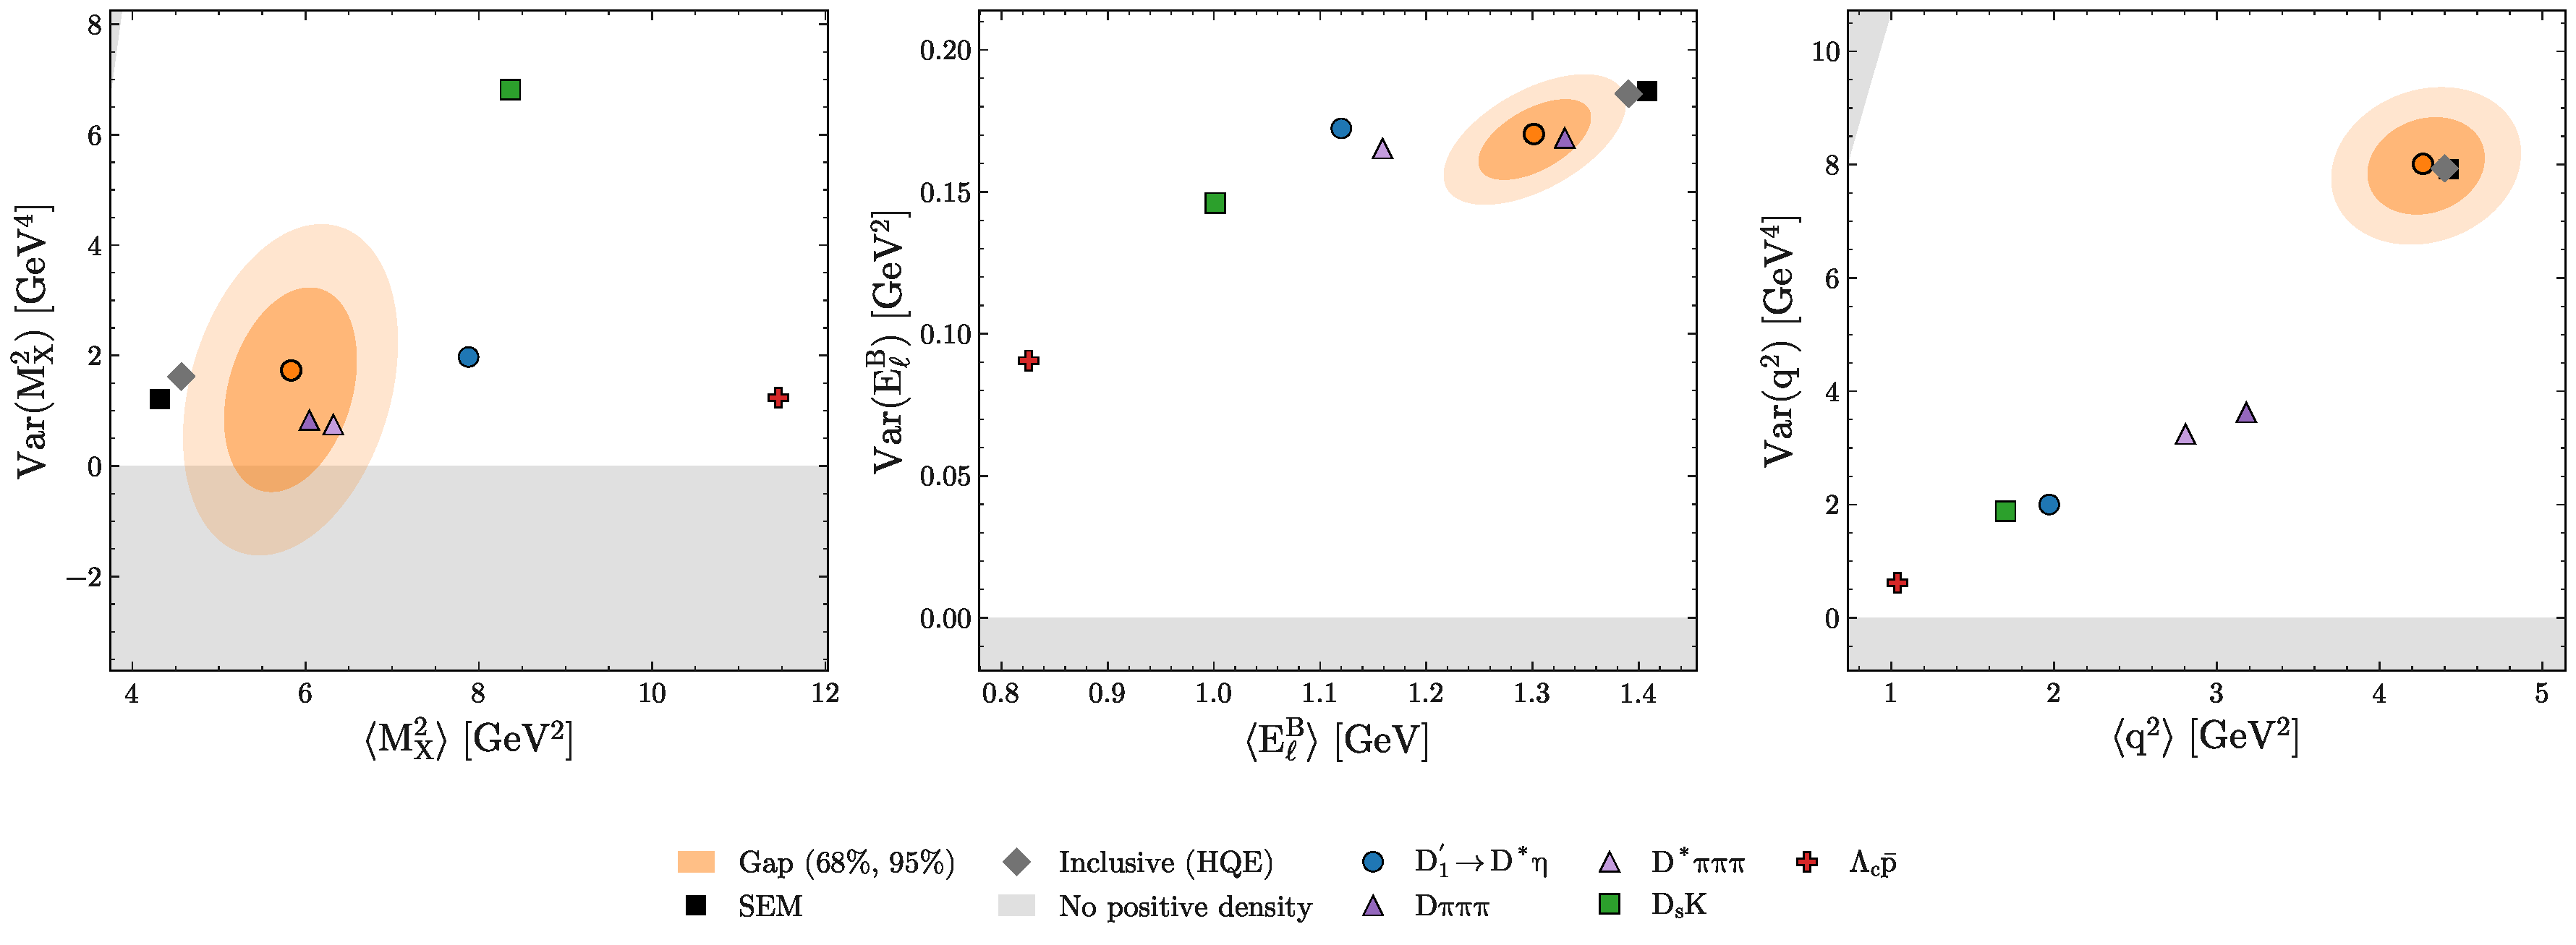
\includegraphics[width=\linewidth]{moment_plane_candidates.pdf}
\caption{As Fig.~\ref{fig:plane}, with candidate gap modes outside the SEM instead of the SEM modes.}\label{fig:plane_cand}
\end{figure}

\FloatBarrier
\subsection{Where the gap can be and how big it must be}
We compute the lowest and highest possible gap CDF over all positive spectra with the measured gap moments
(Fig.~\ref{fig:cdf}). Nothing beyond positivity is assumed. In brackets, the outer edge of the $68\%$ toy range:
\begin{itemize}
\item $\Mx$: $P(\le 8\GeV^2) \ge \nCdfMxEightLo$; $P(\le 10\GeV^2) \ge \nCdfMxTenLo\ (\nCdfMxTenLoToys)$.
\item $\El$: $P(\le 0.5\GeV) \le \nCdfElHalfHi\ (\nCdfElHalfHiToys)$; at least $\nAboveElEight\%$ of the gap has
  $\El > 0.8\GeV$.
\item $q^2$: $P(\le 4\GeV^2)$ between $\nCdfQFourLo$ and $\nCdfQFourHi$; $P(\le 6\GeV^2) \ge \nCdfQSixLo\ (\nCdfQSixLoToys)$.
\end{itemize}
\begin{figure}[htbp]\centering
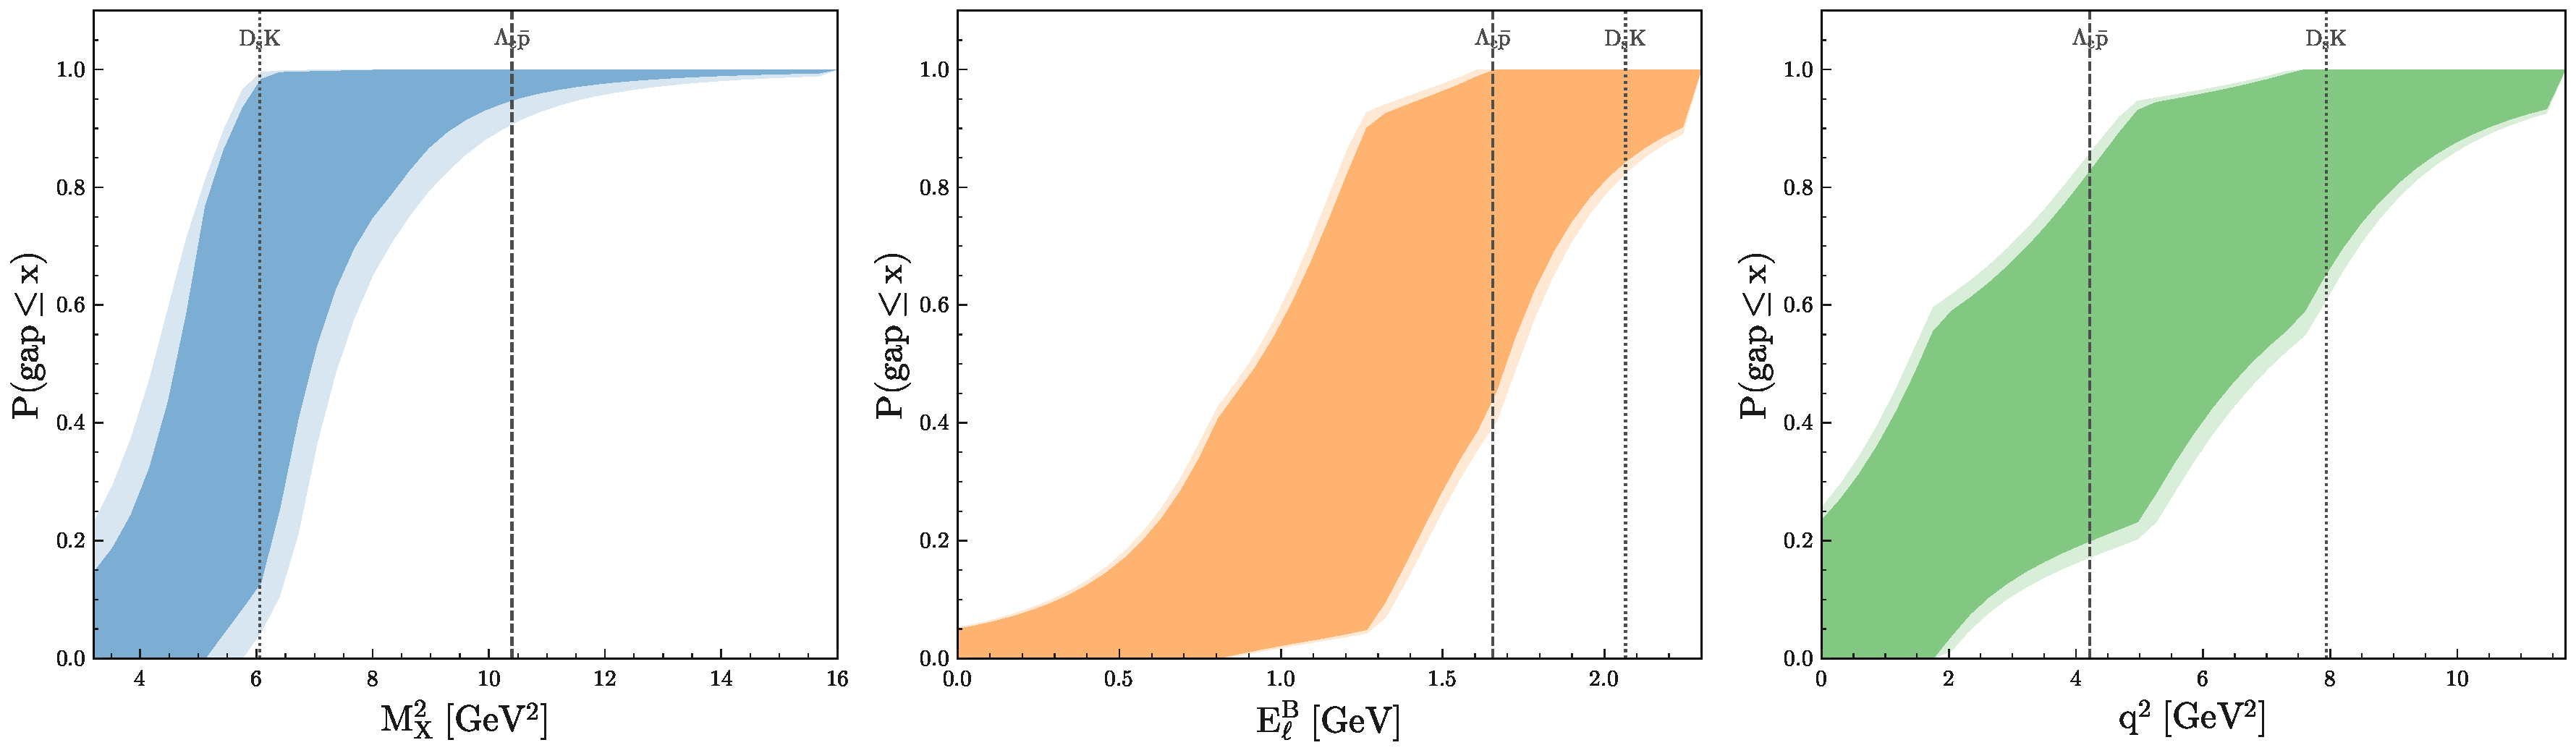
\includegraphics[width=\linewidth]{7/cdf_bounds.pdf}
\caption{Allowed range of the gap CDF (dark) and its $68\%$ toy range (light). Dashed: $\Lcp$ kinematic limit; dotted:
$D_sK$ limit.}\label{fig:cdf}
\end{figure}

The same bounds test whether one class of final states can be the whole gap. \textbf{$\Lcp\ell\nu$ alone is ruled out.}
At least $\nLcpOutMx\%$ of the gap lies below its $\Mx$ threshold ($\nLcpEdgeMx\GeV^2$), and at least $\nLcpOutQ\%$ lies
above its $q^2$ endpoint ($\nLcpEdgeQ\GeV^2$). It is allowed in $\nLcpAllowedMx\%$ of the toys, and $\Mx$ and $q^2$ rule
it out independently. $D_sK\ell\nu$ alone is only disfavoured, by $\Mx$ (allowed in $\nDskAllowedMx\%$ of the toys).

Positivity also needs a minimum gap size. The mean of the inclusive $\Mx$ spectrum lies $\nDMeanMx\GeV^2$ above that of
the SEM. A gap that makes up a fraction $f$ of the rate must therefore sit on average $\nDMeanMx/f\GeV^2$ above the SEM.
That offset spreads the total spectrum by $(1-f)\,\nDMeanMx^2/f$, and this spread must fit into the extra variance of
the inclusive spectrum over the SEM. From the means and variances alone this requires $f \ge \nFMinTwoMoment$; with all
three moments and their uncertainties the $\Mx$ test gives $\BR_\text{gap}/\BR_\text{incl} > \nGapLimitMx$ at $95\%$ CL
(nominal $\nGapFracDec$). $\El$ gives $f > \nGapLimitEl$ and $q^2$ no useful limit. There is no upper limit.
Figure~\ref{fig:size} shows the same scan as the fraction of toys in which a positive gap spectrum exists: for $\Mx$ it is
$\nToyFracNominal\%$ at the nominal size, $50\%$ at $f = \nToyFracHalfAt$ and $\nToyFracAtSeven\%$ at $f = 0.07$. This
fraction is not a confidence level: it asks how often the fluctuated moments are allowed, while the limit asks whether
the measured moments are compatible with allowed ones.
\begin{figure}[htbp]\centering
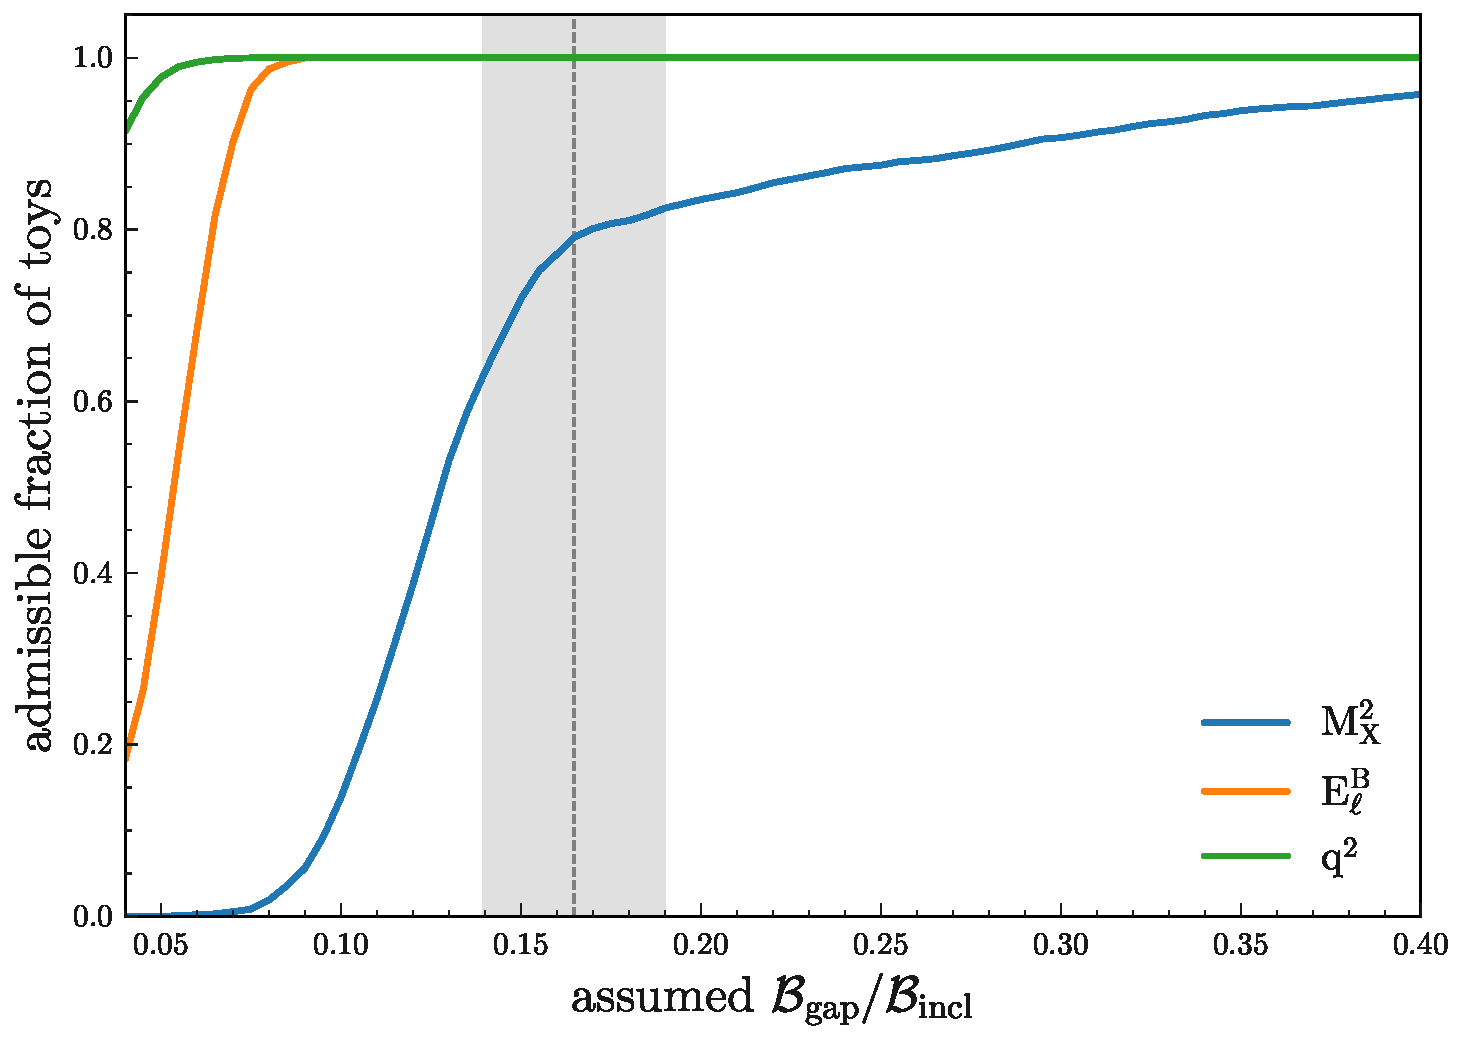
\includegraphics[width=0.55\linewidth]{7/gap_fraction_scan.pdf}
\caption{Fraction of toys in which a positive gap spectrum exists vs the assumed gap size, per observable. Grey band:
the nominal gap size $\pm1\sigma$.}\label{fig:size}
\end{figure}

\FloatBarrier
\subsection{The $\Mx$ moments check MC lineshapes}
With the Belle~II cocktail the SEM has $\mathrm{Var}(\Mx) = \nSemVarMx\GeV^4$, below the inclusive
$\nInclVarMx\pm\nInclVarMxUnc\GeV^4$, and the gap moments are allowed. We then change only the lineshapes of the SEM, at
fixed branching fractions (Table~\ref{tab:lineshape}).
\begin{table}[htbp]\centering\small
\begin{tabular}{>{\raggedright\arraybackslash}p{10.5cm}l}
\toprule
SEM variant & $\Mx$ gap moments \\
\midrule
Belle~II cocktail (nominal) & \nLineshapeAllowed \\
no Hammer weights for broad states & \nLineshapeAllowed \\
HQE $\Mx$ uncertainty doubled & \nLineshapeAllowed \\
$D_1'$:$D_0^*$ split of $D^{(*)}\pi\pi$ from 0 to 1 & \nLineshapeAllowed \\
other kinematic ranges & \nLineshapeAllowed \\
LHCb-style cocktail (ISGW2 $D^{**}$, higher $D^{**}$ states instead of $D^{(*)}\pi\pi$, no $D_sK$) & \nLineshapeAllowed \\
\midrule
$D^{(*)}\pi\pi$ with phase-space lineshape & $d^2 = \nPhspDsq$, $p = \nPhspP$ \\
EvtGen broad states without MCAmbulance & $d^2 = \nBareDsq$, $p = \nBareP$ \\
\bottomrule
\end{tabular}
\caption{Positivity test of the $\Mx$ gap moments for SEM variants with the same branching fractions. $\El$ and $q^2$
are allowed in all variants.}\label{tab:lineshape}
\end{table}

The high-mass tails of the broad states set the SEM $\Mx$ variance, so the test is sensitive to them. The phase-space
model puts too much rate at high $\Mx$ and is rejected ($p < 0.05$) in $\nPhspRejFrac\%$ of the toys. This makes the
inclusive $\Mx$ moments a data-based check of the lineshapes used in inclusive and $R(X)$ analyses. One caveat is still
open: the MC calibration of the measured $M_X$ moments.

Doubling the uncertainty of $\BR_\text{incl}$ (which raises that of $\BR_\text{gap}$ by a factor $\nGInclUnc$) weakens
both rejections, to $p = \nPhspInclP$ for the phase-space lineshape and $p = \nBareInclP$ for the bare EvtGen lineshapes.

\end{document}
